\documentclass{tufte-handout}

\usepackage{ntheorem}
\usepackage{graphicx}
\usepackage{amsmath}
\usepackage{amssymb}
\usepackage{hyperref}
\usepackage{epigraph}
\usepackage{booktabs}
\theoremstyle{break}
% \usepackage[
% bibencoding=utf8,% .bib file encoding
% maxbibnames=3, % otherwise et al
% minbibnames=1, % otherwise et al
% backend=biber,%
% sortlocale=en_US,%
% style=apa,% or authoryear
% % apabackref=false, % backreferences
% natbib=true,% for citet/citep, but this is for backward compatibility
% uniquename=false,%
% url=true,%
% sortcites=false,
% doi=true,%
% eprint=true%
% ]{biblatex}
% \addbibresource{lecture_note_bib.bib}

\hypersetup{
  colorlinks,
  urlcolor = blue,
  pdfauthor={Paul Goldsmith-Pinkham}
  pdfkeywords={econometrics}
  pdftitle={Lecture Notes for Applied Empirical Methods}
  pdfpagemode=UseNone
}
\newtheorem{ruleN}{Rule}
\newtheorem{thmN}{Theorem}
\newtheorem{assN}{Assumption}
\newtheorem{defN}{Definition}
\newtheorem{exmp}{Example}
\newtheorem{cmt}{Comment}
\newtheorem{discussion}{Discussion Questions}
\newtheorem{proof}{Proof}

\newcommand{\continuation}{??}
\newtheorem*{excont}{Example \continuation}
\newenvironment{continueexample}[1]
 {\renewcommand{\continuation}{\ref{#1}}\excont[continued]}
 {\endexcont}
\newcommand{\bY}{\mathbf{Y}}
\newcommand{\bX}{\mathbf{X}}
\newcommand{\bD}{\mathbf{D}}
\newcommand{\E}{\mathbb{E}}

\newcommand\independent{\protect\mathpalette{\protect\independenT}{\perp}}
\def\independenT#1#2{\mathrel{\rlap{$#1#2$}\mkern2mu{#1#2}}}
\DeclareMathOperator{\Supp}{Supp}

\usepackage{cleveref}
\crefname{appsec}{appendix}{appendices}
\crefname{appsubsec}{appendix}{appendices}
\crefname{assumption}{assumption}{assumptions}
\crefname{equation}{equation}{equations}
\crefname{exmp}{example}{examples}
\crefname{assN}{assumption}{assumptions}
\crefname{cmt}{comment}{comments}
\crefname{defN}{definition}{definitions}

\usepackage[nolist]{acronym}
\begin{acronym}
  \acro{CI}{confidence interval}%
  \acro{OLS}{ordinary least squares}%
  \acro{CLT}{central limit theorem}%
  \acro{IV}{instrumental variables}%
  \acro{ATE}{average treatment effect}%
  \acro{RCT}{randomized control trial}%
  \acro{SUTVA}{stable unit treatment value assignment}
  \acro{VAM}{value-added model}%
  \acro{LAN}{locally asymptotically normal}%
  \acro{DiD}{difference-in-differences}%
  \acro{OVB}{omitted variables bias}
  \acro{FWL}{Frisch-Waugh-Lovell}
  \acro{DAG}{directed acyclic graph}
  \acro{PO}{potential outcomes}
\end{acronym}

\def\inprobHIGH{\,{\buildrel p \over \rightarrow}\,} 
\def\inprob{\,{\inprobHIGH}\,} 
\def\indistHIGH{\,{\buildrel d \over \rightarrow}\,} 
\def\indist{\,{\indistHIGH}\,}

\usepackage[many]{tcolorbox} 
\definecolor{main}{HTML}{5989cf}    % setting main color to be used
\definecolor{sub}{HTML}{cde4ff}     % setting sub color to be used
\definecolor{sub2}{HTML}{fde9ce}     % setting sub color to be used

\tcbset{
    sharp corners,
    colback = white,
    before skip = 0.2cm,    % add extra space before the box
    after skip = 0.5cm      % add extra space after the box
}                           % setting global options for tcolorbox

\newtcolorbox{boxD}{
    colback = sub, 
    colframe = main, 
    boxrule = 0pt, 
    toprule = 3pt, % top rule weight
    bottomrule = 3pt % bottom rule weight
}


\newtcolorbox{boxF}{
    colback = sub2,
    enhanced,
    boxrule = 1.5pt, 
    colframe = white, % making the base for dash line
    borderline = {1.5pt}{0pt}{main, dashed} % add "dashed" for dashed line
}

\newtcolorbox{boxK}{
    sharpish corners, % better drop shadow
    boxrule = 0pt,
    toprule = 4.5pt, % top rule weight
    enhanced,
    fuzzy shadow = {0pt}{-2pt}{-0.5pt}{0.5pt}{black!35} % {xshift}{yshift}{offset}{step}{options} 
}
\usepackage{colortbl}


\usepackage{tikz}
\usepackage{verbatim}
\usetikzlibrary{positioning}
\usetikzlibrary{snakes}
\usetikzlibrary{calc}
\usetikzlibrary{arrows}
\usetikzlibrary{decorations.markings}
\usetikzlibrary{shapes.misc}
\usetikzlibrary{matrix,shapes,arrows,fit,tikzmark}

\title{Lecture 5 -- Linear Regression 1 -- Inference}
\author{Paul Goldsmith-Pinkham}
\date{\today}


\begin{document}

\maketitle

This lecture note will discuss focus on the simple linear model, and studying various cases for understanding inference. So far we've focused on \emph{identification} -- e.g. what estimands can we know from the data generating process? Now, given estimators for these estimands, we want to discuss uncertainty and inference.

In this lecture note, we'll be dancing around a fundamental tension. Much of the existing literature and approach to inference is model-based, and as a result, you may feel a bit of a bait-and-switch: I promised a lot of design-based discussion, and all of a sudden we're back in the old world.\footnote{Recall that when I talk about design-based inference, I am thinking about treating the potential outcomes as fixed ($Y(1), Y(0)$) and the treatment assignment $D$ as random. Model-based inference, in the context of lecture note, is considering the model $Y = X\beta + D\tau + \epsilon$, and then thinking about the random sampling of the $(Y, X, D)$ creating uncertainty in the estimates. In other words, it's about the variation in $\epsilon | X,D$.}

The reason for this is that the model-based world is a useful starting point for understanding the basic ideas of inference. A lot of important statistical ideas will show up in this setting,  and it's also the world that most of the literature is written in, so it's important to understand the basic ideas. Overall, just think of these different approaches as different tools in your toolbox.

\section{Review: random sampling and linear regression}
To fix notation, I want to do a refresher on notation and concepts about random sampling. This section is heavily based on review of materials from Gary Chamberlain, to which I am very grateful.\footnote{Gary Chamberlain was an extraordinary econometrician and former teacher of mine who had an amazing set of lecture notes that I got permissiont to \href{https://github.com/paulgp/GaryChamberlainLectureNotes/tree/main}{post online.}} Conceptually, we have considered random variables $(Y, X, D)$ from a joint distribution $F$:
\begin{equation}
  (Y, X, D) \sim F.
\end{equation}

Now, we will formalize the concept of the data we observe that approximates the full population. We'll consider a sample of size $n$, where the $i$th draw of the data gives us the variables $(Y_{i}, X_{i}, D_{i})$.\footnote{In panel settings, with $T$ observations, it is easy to consider $Y_{i}$ being a vector of $Y_{i1}, Y_{i2}, \ldots, Y_{iT}$, and similarly for the other variables. Then, these vectors will be treated as a unit.} We will initially consider random sampling where each draw is independent and identically distributed (i.i.d.):
\begin{equation}
  (Y_{i}, X_{i}, D_{i}) \overset{i.i.d.}{\sim} F.
\end{equation}

Notationally, I'll often group $W_{i} = (X_{i}, D_{i})$\footnote{When I need to make a distinction, $X$ will usually denote controls and $D$ will be the causal variable(s) of interest.} in order to focus on a single set of non-outcome variables. 
The random sampling happens jointly -- we make no distinctions between $Y$ and $W$ in the sampling process. We make that distinction later when we consider the conditional expectation of $Y_{i}$ conditional on $W_{i}$. We will then stack the data $Y_{n} = (Y_{1}, \ldots, Y_{n})$, $W_{n} = (W_{1}, \ldots, W_{n})$. 

We consider the linear predictor
\begin{equation*}
E^{*}(Y_{i}|  W_{i}) = W_{i}'\beta 
\end{equation*}
where $E^{*}$ denotes the linear predictor such that $\beta$ are the minimizer of the expected squared error loss $E((Y- E^{*}(Y_{i}|  W_{i}))^{2})$.\footnote{Note that this is the traditional OLS estimator, and if we want to allow for more flexible functional forms of $W_{i}$, we'll need to include higher-order interactions and functions, etc. } I will assume $W_{i}$ includes a constant for purposes of linear regression. 

Then, recall that
\begin{equation*}
  \beta = E(W_{i}W_{i}')^{-1}E(W_{i}Y_{i}).
\end{equation*}
Note that $\beta$ is a population object, defined based on two moments.

Next recall that the least-squares estimator of $\beta$ is
\begin{align}
  b(Y_{n}, W_{n}) &= \left(n^{-1}\sum_{i=1}^{n}W_{i}W_{i}'\right)^{-1}\left(n^{-1}\sum_{i=1}^{n}W_{i}Y_{i}\right)\\
  &= (W_{n}'W_{n})^{-1}W_{n}'Y_{n}.
\end{align}
Recall that $b$ is a \emph{function} of random variables $Y_{n}$ and $W_{n}$ (an \underline{estimator}) and as such also a random variable. Since we can't directly study $E(b)$, we study instead $E(b | W_{n})$, which focuses on the conditional distribution of $Y_{i} | W_{i}$.\footnote{Why can't we study $E(b)$? The non-linearity makes it hard to study expectations -- the expectation of a ratio is not equal to the ratio of expectations.}

If we consider $E(b(Y_{n}, W_{n}| W_{n} = w))$, we see
\begin{equation*}
  E(b(Y_{n}, W_{n}| W_{n} = w)) = (w'w)^{-1}w'E(Y_{n}| W_{n} = w).
\end{equation*}
When we are correctly specified, and the conditional expectation $E(Y_{n} | W_{n}) = W_{n}\beta$, then we have:
\begin{equation*}
  E(b(Y_{n}, W_{n}| W_{n} = w)) = \beta. 
\end{equation*}
Since this is true for any $w$, we can use the law of iterated expectations and $E(E(b(Y_{n}, W_{n}| W_{n} = w))) = \beta$.

We will now turn to inference in this setting.

\section{Model-based inference}

Given our linear project, $E^{*}(Y_{i} | W_{i}) = W_{i}'\beta$, we write 
\begin{equation*}
  Y_{i} = W_{i}'\beta + \epsilon_{i},
\end{equation*}
where $\epsilon_{i}$ denotes the error term that is mechanically orthogonal to $W_{i}$. As we saw above, we'll often consider the uncertainty in the sampling \emph{conditional} on $W_{i}$, and hence the uncertainty that drives our estimate is from $\epsilon_{i}$ (the unexplained part of $Y_{i}$). Restating our estimator from before, 
\begin{equation*}
  \hat{\beta} = \beta + (\mathbf{W}_{n}'\mathbf{W}_{n})^{-1}\mathbf{W}_{n}'\boldsymbol{\epsilon}_{n}.
\end{equation*}

Typically we take $\mathbf{W}_{n}$ as given, and so the uncertainty (in the model based world) is driven by $\boldsymbol{\epsilon}_{n}$.

Now we consider the variance of $\hat{\beta}$. Formally, we see that this revolves around the structure of $\mathbb{E}(\boldsymbol{\epsilon}_{n}\boldsymbol{\epsilon}_{n}'|\mathbf{W}_{n}) = \Omega_{n}$:
\begin{align}
  \mathbb{V}(\hat{\beta} |\mathbf{W}_{n}) &= (\mathbf{W}_{n}'\mathbf{W}_{n})^{-1}\mathbf{W}_{n}'\mathbb{E}(\boldsymbol{\epsilon}_{n}\boldsymbol{\epsilon}_{n}'|\mathbf{W}_{n})\mathbf{W}_{n} (\mathbf{W}_{n}'\mathbf{W}_{n})^{-1}\\
  &= (\mathbf{W}_{n}'\mathbf{W}_{n})^{-1}\mathbf{W}_{n}'\Omega_{n}\mathbf{W}_{n} (\mathbf{W}_{n}'\mathbf{W}_{n})^{-1}
\end{align}
Everything pivots around the structure of
$\mathbb{E}(\boldsymbol{\epsilon}_{n}\boldsymbol{\epsilon}_{n}'|\mathbf{W}_{n}) = \Omega_{n}$. 

So far, we have assumed that the draws are independent, so we already know that $\Omega_{n}$ is a diagonal matrix.\footnote{Why? Verify this for yourself if this is not clear.} To simplify further, we can consider is homoskedasticity, where $\Omega = \sigma^{2}I_{n}$. This simplifies our variance:
\begin{equation}
  \mathbb{V}(\hat{\beta})_{homoskedastic} = \sigma^{2} (\mathbf{W}_{n}'\mathbf{W}_{n})^{-1}
\end{equation}
What is the content of this assumption? Beyond $Cov(\epsilon_{i},\epsilon_{j}) = 0$, it assumes $Var(\epsilon_{i} |W_{i}) = Var(\epsilon_{i})$.\footnote{This means that conditional on $W=w$, the variance of $Y$ is the same, regardless of the value of $w$. That's pretty strong.}

\begin{boxF}
\begin{cmt}
  \label{cmt:heteroskedasticity_design}
  Consider the linear regression model when posed as potential outcomes with unobserved heterogeneity and strong ignorability:
  \begin{align*}
    Y_{i} &= \alpha + D_{i}\beta + \epsilon_{i}\\
    \alpha &= E(Y_{i}(0))\\
    \beta &= E(Y_{i}(1)) - E(Y_{i}(0))\\
    \epsilon_{i} &= D_{i}\bigg(\underbrace{(Y_{i}(1) - Y_{i}(0))}_{\beta_{i}} - \beta\bigg)  + \bigg(Y_{i}(0) - E(Y_{i}(0))\bigg).
  \end{align*}
Hence, the assumptions about $Var(\epsilon_{i} | D_{i})$ relate directly the extent of heterogeneity in the treatment effect.
Namely, 
\begin{align}
  Var(\epsilon_{i} |D_{i} = 1) &= Var(\beta_{i} | D_{i} = 1) + Var(Y_{i}(0)|D_{i} = 1)\\
  Var(\epsilon_{i} |D_{i} = 0) &=  Var(Y_{i}(0)|D_{i} = 0).
\end{align}
These can only satisfy homoskedasticity and be equal if $Var(\beta_{i}) = 0$, and hence the treatment effect is constant. Under random assignment, the latter terms are equal by construction.
\end{cmt}
\end{boxF}
A feasible estimator for the homoskedastic variance estimand, where $k$ is the number of regressors in $\beta$ (excluding  the constant), follows using empirical analogs:
\begin{equation}
  \label{eq:homoskedastic}
  \hat{\mathbb{V}}(\hat{\beta})_{homoskedastic} = \hat{\sigma}^{2} (\mathbf{W}_{n}'\mathbf{W}_{n})^{-1}  \qquad \hat{\sigma}^{2} = (n-k-1)^{-1}\boldsymbol{\hat{\epsilon}}_{n}' \boldsymbol{\hat{\epsilon}}_{n} 
\end{equation}

If we instead want to allow $Var(\epsilon_{i} | W_{i}) = \sigma^{2}(W_{i})$ to vary with $W$, this implies a potentially complicated function $\sigma^{2}(W_{i})$. But, as it turns out, the estimator for $\mathbb{V}(\hat{\beta})$ is quite straightforward. This is often referred to as the ``robust'' or EHW estimator \citep{eicker1963asymptotic, huber1967behavior, white1980heteroskedasticity}:
\begin{equation*}
  \hat{\mathbb{V}}(\hat{\beta})_{EHW} = (\mathbf{W}_{n}'\mathbf{W}_{n})^{-1}\sum_{i}\hat{\epsilon}_{i}^{2}W_{i}W_{i}'(\mathbf{W}_{n}'\mathbf{W}_{n})^{-1}.
\end{equation*}

\begin{boxD}
\begin{exmp}
  \label{exmp:binary}
  Consider the case where $W_{i} = (1, D_{i})$, and $D_{i}$ is a dummy treatment variable. Then, the variance of the coefficient on $D_{i}$ reduces to
\begin{equation*}
       \hat{\mathbb{V}}(\hat{\beta})_{homoskedastic} = \frac{\hat{\sigma}^{2}}{n_{0}} + \frac{\hat{\sigma}^{2}}{n_{1}} = \frac{\hat{\sigma}^{2}}{n}, \qquad \hat{\mathbb{V}}(\hat{\beta})_{EHW} = \frac{\hat{\sigma}^{2}(0)}{n_{0}} + \frac{\hat{\sigma}^{2}(1)}{n_{1}},
     \end{equation*}
where $n_{0} = \sum_{i} (1-D_{i})$, $n_{1} = \sum_{i} D_{i}$ and $\hat{\sigma}^{2}(x)$ is the estimated variance of $\epsilon_{i}$ for observations with $D_{i} = x$. 
    \end{exmp}
  \end{boxD}

We then consider confidence intervals based around distributional assumptions. Recall that our distributional assumptions come from considering the following statistics: 
\begin{equation*}
  T = \frac{\hat{\beta} - \beta}{\sqrt{\hat{\mathbb{V}}/\nu}}
\end{equation*}

When we assume that the distribution of $\epsilon$ is homoskedastic and Normal, we know the exact distribution of $T$. That's because $\beta$ is consequently the sum of independent normals, and the variance of $\hat{\beta}$ is a scaled chi-squared (since a squared normal is chi-squared). This is the basis for the $t$-distribution.\footnote{E.g. $T = Z / \sqrt{V/\nu}$, where $Z \sim \mathcal{N}(0,1)$, $V \sim \chi^{2}(\nu)$}

Without homoskedastic Normality, the distribution for $T$ is only Student-$t$ asymptotically. This approximation works pretty well in many settings, but there are edge cases where issues can arise.\footnote{Edge cases that you likely know well include weak IV and unit roots. I call them edge cases because they usually involve sending a parameter to a boundary case, such as the first-stage coefficient to zero, or AR parameter to one.} One straightforward edge case we'll consider now is when $n_{1}$ and $n_{0}$ are not both simultaneously growing large.

\subsection{Confidence intervals, finite sample performance, and the Behrens-Fisher problem}
Note that in our discussion above, the feasible estimator for $\hat{\sigma}^{2}(x)$ was not made explicit. For the homoskedastic case, we have a simple estimator in \Cref{eq:homoskedastic}. We have adjusted for $k$ in this estimator to account for the bias that arises from our estimation of $\beta$. A similar adjustment needs to occur for the heteroskedastic case to account for the estimation of the parameters as well. Note that this is a \emph{finite sample} adjustment, since it will not matter as $n$ gets large.

It is worth highlighting the different relevant adjustments that get made in the heteroskedastic case, which will matter for practical inference.\footnote{See the discussion in \Cref{cmt:packages_robust} for implementations, and the implications of using biased estimators in \Cref{fig:imbenskolesar_simulation}.} The original EHW estimator is biased, and does not adjust for the $k$ parameters. \citet{mackinnon1985some} propose a second estimator, referred to as the HC2 estimator, that adjusts for the bias in the variance estimator.\footnote{There is also a third estimator, referred to as HC3, from \citet{mackinnon2012thirty}, that also adjusts for the bias in the variance estimator. It is quite conservative (it's biased upwards in the case of binary treatment). For the binary case, it is given by
\begin{equation*}
  \hat{\mathbb{V}}(\hat{\beta})_{EHW} = \hat{\sigma}^{2}(0)\frac{n_{0}}{(n_{0}-1)^{2}} + \hat{\sigma}^{2}(1)\frac{n_{1}}{(n_{1}-1)^{2}}.
\end{equation*}
I provide it for completeness, but it is not widely used.}
It's exactly unbiased in the binary treatment case, but this is not generally true. In the binary case, it adjusts simply by subtracting one:
\begin{equation*}
  \hat{\sigma}^{2}(d) = \frac{1}{n_{d} -1}\sum_{i}D_{i} (Y_{i} - \overline{Y}_{d})^{2}.
\end{equation*}

So far, we have just discussed different estimators for $\mathbb{V}$. Recall that we want to use these to make confidence intervals, based on the distribution of $T$. That distribution requires an assumption about the degrees of freedom for $T$. Then, we can construct 95\% confidence intervals based on these asymptotic results:
\begin{align*}
\text{CI} &= \left(\beta - t^{n-2}_{0.975}\times \sqrt{\hat{\mathbb{V}}}, \beta + t^{n-2}_{0.975}\times \sqrt{\hat{\mathbb{V}}}\right)
\end{align*}
where $t^{n}_{q}$ is the $q$th quantile the $t$ distribution with degrees of freedom $n$. The issue is that the degrees of freedom are not clear in the heteroskedastic case. Why? Because the variance is the weighted sum of \emph{different} Chi-squared distributions. This is very concrete in \Cref{exmp:binary}, where the denominator of the scaling for the variance is driven by the relative size of the treatment and control groups.

We now consider the Behrens-Fisher problem. Imagine that $n_{0} >> n_{1}$, that is, there are few treated units relative to the control.\footnote{These results and discussion come from \citet{imbens2016robust}.}  Then, the distribution is really driven by $\sigma^{2}(1)/n_{1}$, and $n_{1}$ is the correct degrees of freedom. This makes a big difference! Contrast the degrees of freedom between the two cases: $t^{3}_{0.975} = 3.182$  vs. $t^{28}_{0.975}=2.048$.\footnote{Notably, this issue starts to disappear as the minimum size  gets large.} This naturally creates much wider confidence intervals for a given dataset, which implies that the coverage under the $n_{0}$ degrees of freedom would have much lower coverage than the $n_{1}$ degrees of freedom. We can see this coverage difference in simulations done by \citet{imbens2016robust} in \Cref{fig:imbenskolesar_simulation}.
      

\begin{figure}
  \label{fig:imbenskolesar_simulation}
    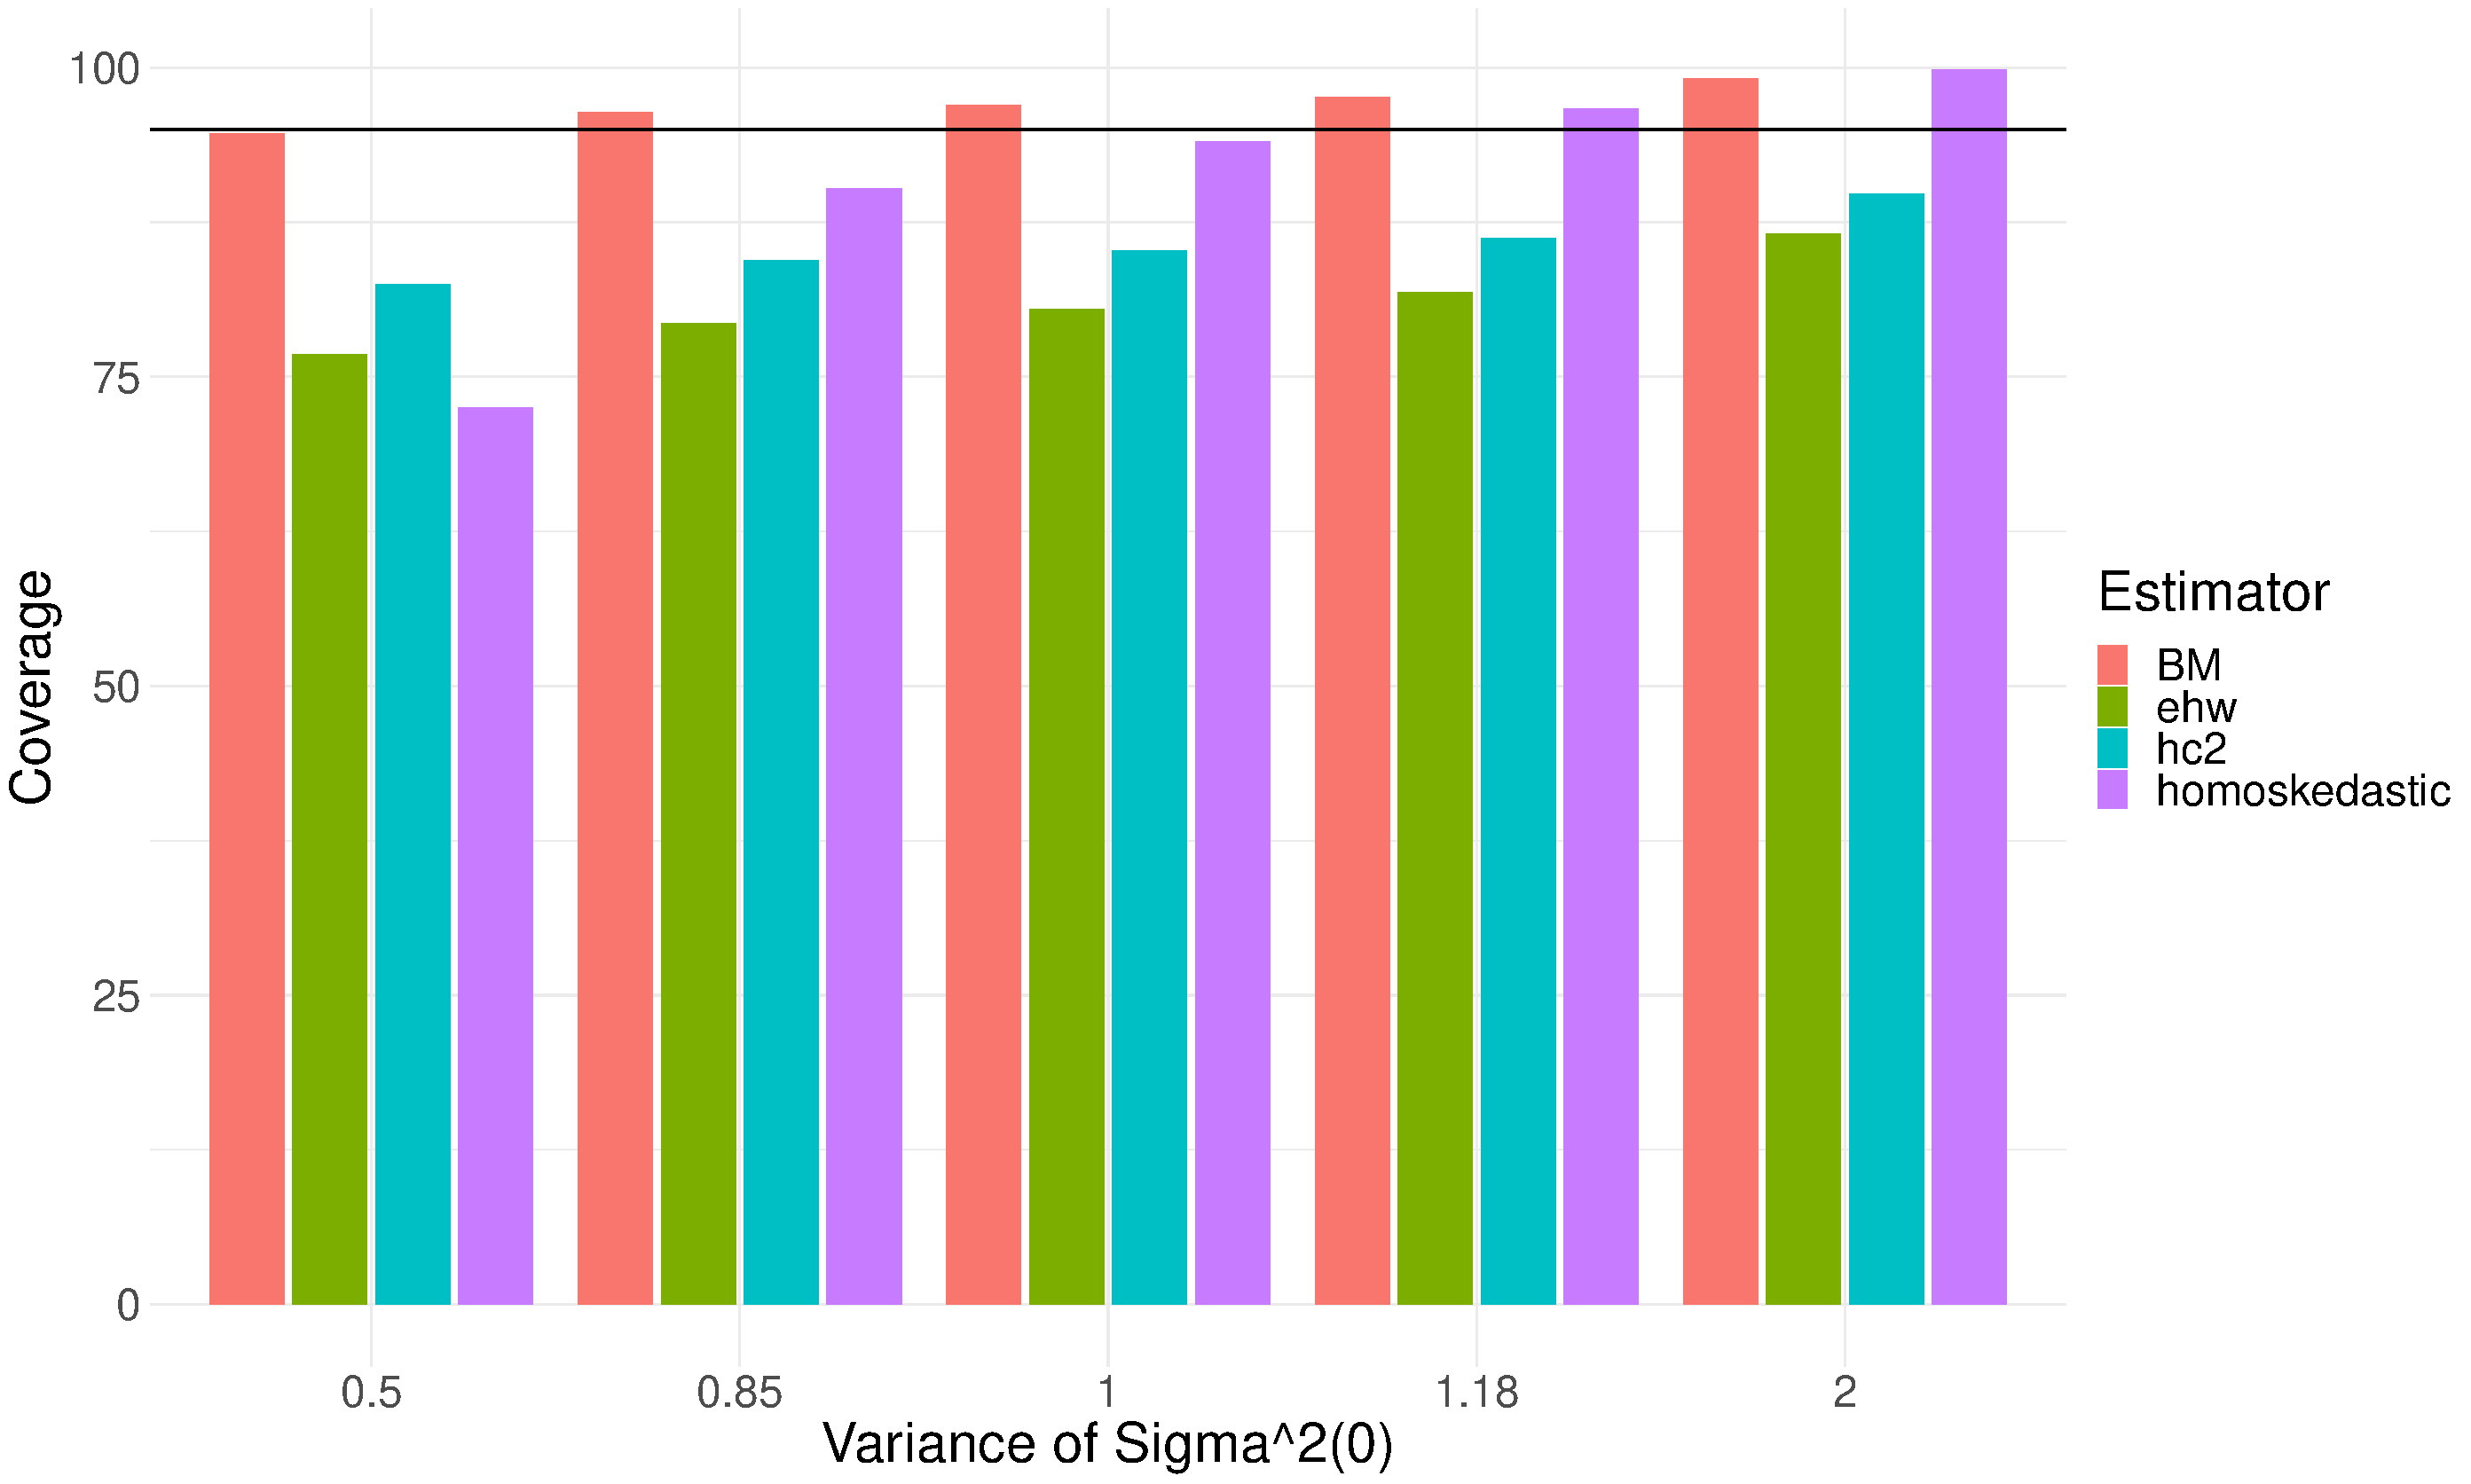
\includegraphics[width=\linewidth]{../lectures/images/imbenskolesar_coverage.pdf}
    \caption{
      These simulation results come from \citet{imbens2016robust} and study the impact of unbalanced treatment and control. In the simulation, $n=30, n_{0} = 27, n_{1} = 3$. The coverage of the different estimators discussed in \Cref{cmt:robust} are shown. The Bell-Maccaffrey adjustments are the most accurate, and EHW does poorly in all cases. The data is simulated to be Normally distributed conditional on treatment, and the Variance of the error term is allowed to vary.
      }
    \end{figure}
 
The estimator with the best performance in this setting is the Bell-Maccaffrey adjustment, which is a generalization of the HC2 estimator. This estimator adjusts for the degrees of freedom issue by finding the parameter $K$ which creates a $t$-distribution that most closely matches the first two moments of the dispersion of the estimated $\hat{V}_{HC2}$ around the estimand.\footnote{This is done under the assumption of homoskedasticity, for \emph{just} the purposes of estimating the degrees of freedom.} In the binary case, this reduces to 
\begin{equation*}
  K_{BM} = \frac{(n_{0} + n_{1})^{2}(n_{0}-1)(n_{1}-1)}{n_{1}^{2}(n_{1}-1)+n_{0}^{2}(n_{0}-1)}.
\end{equation*} 
Some intuition arises in the case when $n_{0}$ and $n_{1}$ are similar: we get $K_{BM} = n-2$, which is the degrees of freedom in the homoskedastic case. If $n_{0} >> n_{1}$, then we get $K_{BM}  \approx n_{1}$. This is a very intuitive result, and lines up with what we'd want. \citet{imbens2016robust} recommend this estimator to researchers in practice.

The Behrens-Fisher issue (and Bell-Maccaffrey solution) generalizes to general regression setting, even when the treatment is not binary. The key idea is that the variance we're scaling by is not a Chi-squared with the full degrees of freedom $n$. The approximation that we use matches the degrees of freedom to get the first and second moment as close as possible to the ``right'' chi-squared.\footnote{These issues can rear their head when the the regressor of interest is highly skewed (e.g. a log-normal right hand side variable). The intuition comes from the fact that the distribution of the regression will affect the distribution of $(W_{n}'W_{n})^{-1}W_{n}'\epsilon_{n}$, warping the finite sample behavior of the sum of the $\epsilon_{n}$ sum.}


\begin{boxF}
\begin{cmt}
\label{cmt:packages_robust}
What are the statistical packages that we use in these cases, and what's doable?

\begin{itemize}
  \item Stata uses the EHW standard errors by default (with the \texttt{robust} command). But, I believe as of Stata 17, it does the correct finite sample adjustment for the degrees of freedom to make it unbiased in the simple case. You can use \texttt{vce(hc2)} to get the HC2 estimator, and \texttt{vce(hc3)} to get the HC3 estimator. For the Bell-Maccaffrey adjustments,
  see \texttt{reg\_sandwich}.
  \item In R, there are many pacakges, but the ones I would look see \texttt{estimatR},
          \texttt{clubSandwich}, and \href{https://github.com/kolesarm/Robust-Small-Sample-Standard-Errors}{Kolesar's github repo.}
\end{itemize}
        \end{cmt}
      \end{boxF}        

\begin{boxD}
  \begin{exmp}
    You might be asking yourself, why do I have to care about these things? For a lovely discussion of finite sample issues, you should peruse \href{https://datacolada.org/99}{Data Colada's discussion} of \href{https://academic.oup.com/qje/article/134/2/557/5195544?login=true}{Alwyn Young's QJE paper on randomization inference}. The paper is a great example of how finite sample issues can matter in practice.

    \hspace{10pt}To quote the post:
    ``In this post I show that this conclusion only holds when relying on an unfortunate default setting in Stata. In contrast, when regression results are computed using the default setting in R [1], a setting that's also available in Stata, a setting shown over 20 years ago to be more appropriate than the one used by Stata... the supposed superiority of the randomization test goes away.''
  \end{exmp}
  \end{boxD}

\paragraph{Bootstrap}    One nice alternative approach to distributional assumptions on $T$ is to use the bootstrap. The bootstrap is a general purpose tool for constructing confidence intervals, and it can be used in the context of linear regression. The idea is to resample the data with replacement, and then re-estimate the model. This comes in many forms, but the most intuitive and straightforward form is called the non-parametric bootstrap, which would involve resampling $n$ observations of $(Y_{i}, W_{i})$ from the data with replacement, and then re-estimating the model. After $B$ samples are re-estimated, this will give us a distribution of the parameter and we can describe the statistical properties of this distribution (e.g. the 95\% interval of this distribution). It is also plausible to construct t-statistics $t_b = (\hat{\beta}_{b}-\beta^{0})/\sqrt{V_{b}}$ for each bootstrap sample $b$ and null hypothesis $\beta^{0}$, and use this instead of $\hat{\beta}$. Since the $t$-statistic is asymptotically pivotal, it can have nice properties. 

However, the non-parametric bootstrap can have issues if the sample is small or the regressors are skewed \citep{imbens2016robust}, as the additional noise introduced by resampling creates worse distributional approximations. One very successful bootstrap alternative is the wild bootstrap. Concretely, this works as follows (see \citet{DAVIDSON2008162} for details):
    \begin{enumerate}
      \item Estimate the linear model $\hat{\beta}$ and obtain residuals $\hat{\epsilon}_{i}$.
      \item In each bootstrap step $b$:
      \begin{enumerate}
        \item For each observation $i$, the $X_{i}$ is fixed, along with $\hat{\beta}$ and $\hat{\epsilon}_{i}$. We then draw a binary variable $U_{i,b}$ that is either $1$ or $-1$ with equal probability. We set $Y_{i,b} = \hat{\beta}X_{i} + U_{i,b}\hat{\epsilon}_{i}$.
        \item With the new dataset, we re-estimate the model and construct a t-statistic $t_{b}^{1} = (\hat{\beta}_{b}-\hat{\beta})/\sqrt{\hat{V}_{b}}$, where $\sqrt{\hat{V}_{b}}$ is the standard error.
      \end{enumerate}
      \item With the full set of $t_{b}$, we can construct a confidence interval by calculating the $q_{0.95}(|t_{b}|)$, the 0.95 quantile of $|t_{b}|$, and using it in the place of our usual critical value:
      \begin{equation*}
        \text{CI}_{WILD} = \left(\hat{\beta} - q_{0.95}(|t_{b}|)\sqrt{\hat{V}}, \hat{\beta} + q_{0.95}(|t_{b}|)\sqrt{\hat{V}}\right)
      \end{equation*}
    \end{enumerate}


\section{Combining Sampling- and Design-based uncertainty }

How should we be thinking about inference anyway? What's the error in $\epsilon$ \emph{mean}? The thought experiment typically comes from a sampling perspective -- we consider that this is a small sample from a broader population, and uncertainty comes from whether the estimates reflect the true underlying population. Note that this contrasts with our design-based thought experiment!

This starts to get very confusing when thinking about some settings. For example, how do we think about sampling ``new states'' when we have all 50 states? Worse yet, what if we have access to all the census data? We observe the whole population! What's the uncertainty in our estimates then? In estimation of causal effects, we still  uncertainty because there's uncertainty driven by the  fundamental problem of causal inference!

Using work from \citet{abadie2020sampling}, we will now consider two sources of uncertainty: sampling and design. There exists a population of size $N$ and a sample of size $n \leq N$.\footnote{My $n,N$ are reversed from the paper.} Let $R_{i} = \{0,1\}$ denotes whether or not an observation is in the sample.  There are also potential outcomes $Y^{*}(D_{i})$.  Now we have both sampling uncertainty (e.g. does our sample reflect the population) and design uncertainty (e.g. does the causal comparison reflect the true causal effect). We can now combine the two sources of uncertainty to get a better understanding of the variance of our estimator.

I will focus on just binary case of a single treatment, but the paper considers full regression setting. We consider three estimands:
\begin{enumerate}
  \item $\theta^{descr} = N^{-1}_{1}\sum_{i=1}^{N}D_{i}Y_{i} - N^{-1}_{0}\sum_{i=1}^{N}(1-D_{i})Y_{i}$
  \item $\theta^{causal, sample} = n^{-1}\sum_{i=1}^{N}R_{i}(Y^{*}_{i}(1) - Y_{i}^{*}(0))$
  \item $\theta^{causal} = N^{-1}\sum_{i=1}^{N}(Y^{*}_{i}(1) - Y_{i}^{*}(0))$    
\end{enumerate}
We have a single estimator we can consider:
\begin{equation*}
  \hat{\theta} = n^{-1}_{1}\sum_{i=1}^{N}R_{i}D_{i}Y_{i} - n^{-1}_{0}\sum_{i=1}^{N}R_{i}(1-D_{i})Y_{i}
\end{equation*}
The key point of paper -- the variance of this estimator depends on what we condition on. If we condition on  $D$, we focus on sampling uncertainty. If we condition on $R$ we focus on causal uncertainty within sample. If we condition on neither, we focus on causal uncertainty as well as sampling uncertainty.
      
What are these variance estimands? Let $S_{x}$ denote the population variance for each potential outcome, and $S_{\theta}$ denote the population variance of the treatment effect outcomes (which recall, we cannot directly estimate).\footnote{This variance is $S_{\theta} = \frac{1}{N-1}\sum_{i}\left(Y_{i}(1) - Y_{i}(0) - N^{-1}\sum_{i}(Y_{i}(1) -Y_{i}(0))\right)^{2}$.} Then, we have the following variance estimands:
\begin{enumerate}
  \item Sampling: $E(Var(\hat{\theta} | \mathbf{D}, n_{1}, n_{0}) | n_{1}, n_{0}) = \frac{S^{2}_{1}}{n_{1}}\left(1- \frac{n_{1}}{N_{1}}\right) + \frac{S^{2}_{0}}{n_{0}}\left(1- \frac{n_{0}}{N_{0}}\right),$
  \item Design:  $E(Var(\hat{\theta} | \mathbf{R}, n_{1}, n_{0}) | n_{1}, n_{0}) = \frac{S^{2}_{1}}{n_{1}} + \frac{S^{2}_{0}}{n_{0}} - \frac{S^{2}_{\theta}}{n_{1}+n_{0}}    $
  \item Both: $Var(\hat{\theta} | n_{1}, n_{0}) = \frac{S^{2}_{1}}{n_{1}} + \frac{S^{2}_{0}}{n_{0}} - \frac{S^{2}_{\theta}}{N_{1}+N_{0}}    $
\end{enumerate}
The $S^{2}_{\theta}$ term is what we usually ignore (because not feasibly estimable). Consider the following thought experiments: let $n$ get close to $N$, or let $n$ get small relative to $N$. This will move around the sampling and total variance estimands, but not the sample causal estimand. Next, notice that the difference between Sampling and Design is not obvious. Sampling can be small if $n$ is close to $N$, but when $S_{\theta}^{2}$ is large, that can make the design variance small.

\section{Clustering and generalizing $\Omega$}
This ignored any sort of unusual correlation structure in $\Omega$, and assumed random assignment.
 In many cases, we don't have that. Instead, $\Omega$  has a clustering structure. This can get quite complex. Let's start with the simple case of known clusters. E.g. units are people, and clusters are cities, counties or states. For today, we're ignoring the very important question of panel data. We'll come back to that later.

Let $C_{i}$ denote unit $i$'s cluster assignment. A very simple version of $\Omega$ is now
\begin{equation}
  \label{eq:clustering}
\Omega_{ij}  =\left \{\begin{array}{ccc}
      \sigma^{2} &  \text{if}& i = j\\
      \rho\sigma^{2}  & \text{if}&  C_{i} = C_{j} \; \& \; i \not= j\\
      0 & \text{if} & C_{i} \not= C_{j} \; \& \; i \not= j
    \end{array}\right. 
\end{equation}
This matrix can also be more unstructured. For exmaple, one could have a flexible block diagonal with $\Omega_{ij} = \sigma_{ij}$ if $C_{i} = C_{j}$. A key issue that arises here is in the relative size of the block versus the number of blocks. See \citet{hansen2007asymptotic} for a discussion of one example.

Let's start with a model-based approach to this. Denote the number of clusters by $K$. Following \citet{liang1986longitudinal}, the estimator for the variance of $\hat{\beta}$  is
\begin{equation}
  \hat{\mathbb{V}}(\hat{\beta} |\mathbf{W}_{n}, \mathbf{C}_{n})_{LZ} = (\mathbf{W}_{n}'\mathbf{W}_{n})^{-1}\left(\sum_{k=1}^{K}\mathbf{W}_{k,n}'\hat{\boldsymbol{\epsilon}}_{k,n}\hat{\boldsymbol{\epsilon}}_{k,n}'\boldsymbol{W}_{k,n}\right) (\mathbf{W}_{n}'\mathbf{W}_{n})^{-1}.
\end{equation}

This estimator allows for flexible covariance within the block, and assumes that the size of the block is fixed, and that $K$ is large.\footnote{In fact, the degrees of freedom are defined by the size of $K$.}  Historically, clustering in this setting has focused the structure of $\Omega$. Why? Well, take the simple case  in \Cref{eq:clustering}. In this case,
\begin{equation}
  \mathbb{V}(\hat{\beta}) = \mathbb{V}_{homoskedastic}\times \left( 1+ \rho_{\epsilon}\rho_{W}\frac{n}{K_{n}}\right),
\end{equation}
where $\rho_{\epsilon}$ and $\rho_{W}$ are the within-cluster correlations of each r.v. This makes you think that these are the main terms that matter, and more generally it's about getting the structure of $\Omega$ right. E.g., better to err on the conservative side and let the blocks be large. 

However this intuition is \emph{not} correct in contexts with any meaningful heteroskedasticity.  \citet{abadie2023should} can generate an example with tiny within-cluster
    correlation, and large clusters (with many clusters) where the Liang-Zeger estimator $\hat{\mathbb{V}}(\hat{\beta})_{LZ}$ is large and $\hat{\mathbb{V}}(\hat{\beta})_{EHW}$ is small. How come? Recall from \Cref{cmt:heteroskedasticity_design} that the variance of the error term depends on two pieces: the variance of the poetntial outcome, and the variance of the tratement effect, as it correlates with treatment. Namely, it's all about the correlation \emph{between} $W$ and $\epsilon$, and heterogeneity in our effects across clusters.

In \citet{abadie2023should}, they construct an example where $N = 10,000,000$ with 100 equal sized clusters. There is a binary $W$ with \emph{equal} probability.  THere are significant heterogeneous effects of $W$ across clusters -- some clusters have positive effect, some have negative. Overall ATE is 0. What does that mean intuitively? If there is heterogeneity in effects, it causes correlation between treatment and residual.

So why do the two standard error estimators vary so much? To quote the \citet{abadie2023should} working paper:
\begin{fullwidth}
\begin{quote}
  The reason for the difference between the EHW and LZ standard errors is simple, but
  reflects the fundamental source of confusion in this literature. Given the random assignment
  both standard errors are correct, but for different estimands. The LZ standard errors are based
  on the presumption that there are clusters in the population of interest beyond the 100 clusters
  that are seen in the sample. The EHW standard errors assume the sample is drawn randomly
  from the population of interest. It is this presumption underlying the LZ standard errors of
  existence of clusters that are not observed in the sample, but that are part of the population
  of interest, that is critical, and often implicit, in the model-based motivation for clustering the standard errors. It is of course explicit in the sampling design literature (e.g., Kish [1965]). If we changed the set up to one where the population of 10,000,000 consisted of say 1,000 clusters,
  with 100 clusters drawn at random, and then sampling units randomly from those sampled
  clusters, the LZ standard errors would be correct, and the EHW standard errors would be
  incorrect. Obviously one cannot tell from the sample itself whether there exist such clusters
  that are part of the population of interest that are not in the sample, and therefore one needs
  to choose between the two standard errors on the basis of substantive knowledge of the study
  design.
\end{quote}
\end{fullwidth}

What are the key takeaways from this paper? First, cluster your regression at the unit of randomization. Being conservative can be quite bad! It depends on what you are trying to do.
The traditional advice of being as conservative as necessary is likely misguided. Fixed effects do NOT remove the need for clustering. We'll revisit this in panel settings. 

\begin{boxK}
  \begin{discussion}
    What is the ``unit of randomization'' in a case like \citet{card1994minimum}?
  \end{discussion}
\end{boxK}

    \begin{boxF}
\begin{cmt}[Spatial and Network Error]
  Things get more complicated with more general error structures. Consider two additional cases:
    \begin{itemize}
    \item Spatial correlation = $\rho_{ij} = f(d_{ij})$, where $d_{ij}$ is a function of some economic distance.
    \item Social network correlation = $\rho_{ij} = f(d_{ij})$, where $d_{ij}$ is a function of path length in a network
    \end{itemize}
  This can matter especially when SUTVA is violated
 However, Barrios et al. (2012) show that, under SUTVA, if
    treatments are randomly assigned at a given cluster level, we can
    ignore the broader spatial correlations


Conley (1999) provides a flexible way to consider clustering on spatial distances.
Consider our matrix $\Omega$ again. Now, $\Omega_{ij}$ is a
    function of the distance, $d_{ij}$, between each
    person. Unfortunately, this means that every person can be
    correlated.
Key assumption -- the correlation declines with
    distance. Hence, far away distances matter less in
    practice. Hence, when we estimate this, we ``window'' our
    estimator (this is exactly the same as Newey-West
    estimators). Then we allow correlation as in the Liang-Zeger
    estimator, as a function of distances.
This estimator is consistent for general forms of spatial
    correlation
    \begin{itemize}
    \item Estiators available in both Stata and R
    \end{itemize}
  \end{cmt}
\end{boxF}


\begin{boxD}
  \begin{exmp}
Consequences of ignoring spatial correlation

Spatial correlation can be a big deal. Consider the analogy to time series.
    \begin{itemize}
    \item A big rule: worry about highly autocorrelated data! Can inflate your t-statistics substantially
    \item Why? Because if we treat observations as independent, we
      will infer more information than actually exists
    \end{itemize}
  \item Kelly (2019) claims that spatial correlation in outcomes can
    cause this same issue. Consider a regression of some modern
    outcome, e.g. city income, on a historical characteristic, such as
    colonial boundaries
    \begin{itemize}
    \item Claim in Kelly (2019) is that t-statistics in these types of regressions are grossly amplified by spatial correlation
    \item Fixable with Conley standard errors?
    \item This is a huge deal for a lot of literatures (economic
      history especially) -- matters for corporate governance
      literature too (LLSV)
    \end{itemize}
  \end{exmp}
\end{boxD}
  

\section{Concluding thoughts}
 This stuff is \emph{hard}. We are doing the simplest case
    (linear regression) and still have lots of questions. As always, asking what the knowable estimand is can be very helpful. Next, if you are unsure, it is very useful to consider simulating data. \footnote{This is the approach advocated in \citet{blair2023research}.} 
In many cases, there is not an obvious ``best'' answer, and simulating your data is the best solution. This is because many results are asymptotic in nature, and hence approximations. 


So how does one implement a simulation? Goal is to generate data that matches your dataset's distributions. However, for very simple simulations, you'll have to make
    parametric assumptions that may not match your actual data. 
    Athey et al. (2020) propose a method for matching the data as
    closely as possible, using a Generative Adverserial Network. In other words, construct distributions that match the ``true'' data as
    closely as possible
    \begin{itemize}
    \item Computationally expensive, but great way to evaluate performance
    \item Code is available here: \url{https://github.com/gsbDBI/ds-wgan}
    \item Docs are here: \url{https://github.com/gsbDBI/ds-wgan}
    \end{itemize}

 However this stuff is really hard to implement.
 If you intuitively know the issue, try doing something simple with normals
 Or try bootstrapping!

\begin{figure}
    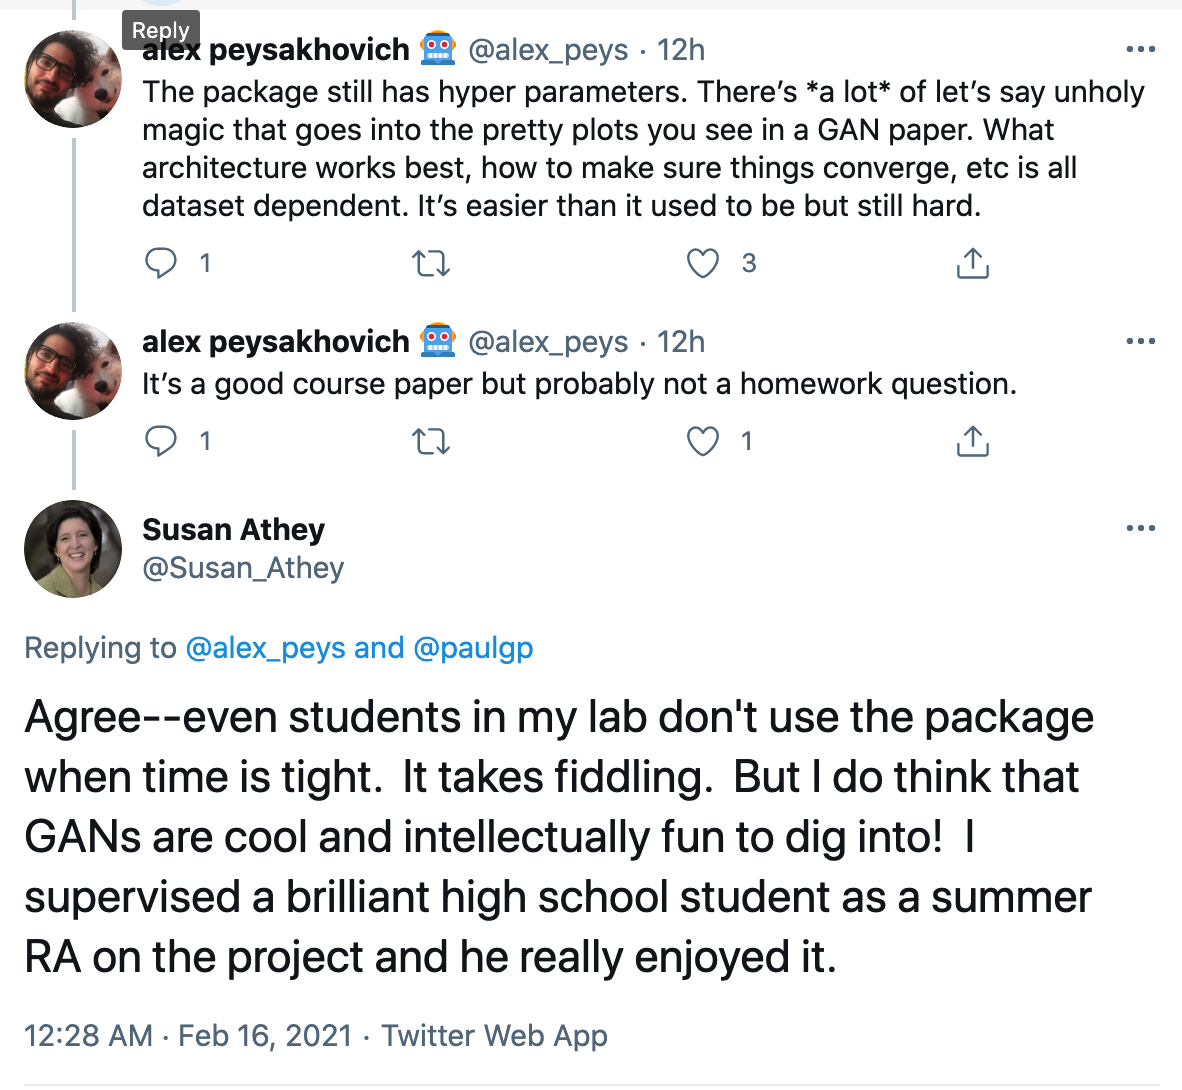
\includegraphics[width=\linewidth]{../lectures/images/gan_fiddle.png}
\end{figure}
      

\bibliography{lecture_note_bib.bib}
\bibliographystyle{plainnat}

\end{document}